\section{Описание модели}

\qquadВ работе рассматривается полностью ионизированная, идеальная неравновесная 
плазма, состоящая из положительно заряженных однозарядных ионов и электронов. 
В токамаках, где поддерживается низкое давление($\sim 10^{-8}$ торр), плазма является неравновесной и температура
электронов много больше температуры ионов и атомов: $T_a \approx T_i < T_e$, отсюда, в модели принято: $T_i = 0$. Электроны, приходящие из плазмы,
всюду находятся в равновесии и имеют распределение Максвелла. Плазма квазинейтральна вплоть
до входа в дебаевский слой: $n_i^{se} = n_e^{se} = n^{se}$.


\qquadСтенка имеет координату $x = 0$, точки, соответствующие слою и
плазме, имеют положительные координаты~\autoref{pic::model}.
На стенке устанавливается квазистационарное равновесие: сумма токов равна 0 и стенка имеет установившийся плавающий потенциал $V_f$, имеющий
характерное значение порядка $eV_{char} = -3T_e$ и эффективно отражающий поток электронов из плазмы. Знак плавающего
потенциала('нуль' потенциала принят на $x\rightarrow + \infty$) 
и монотонность электростатического потенциала в
слое определяются режимом работы слоя.

\begin{figure}
	\centering
	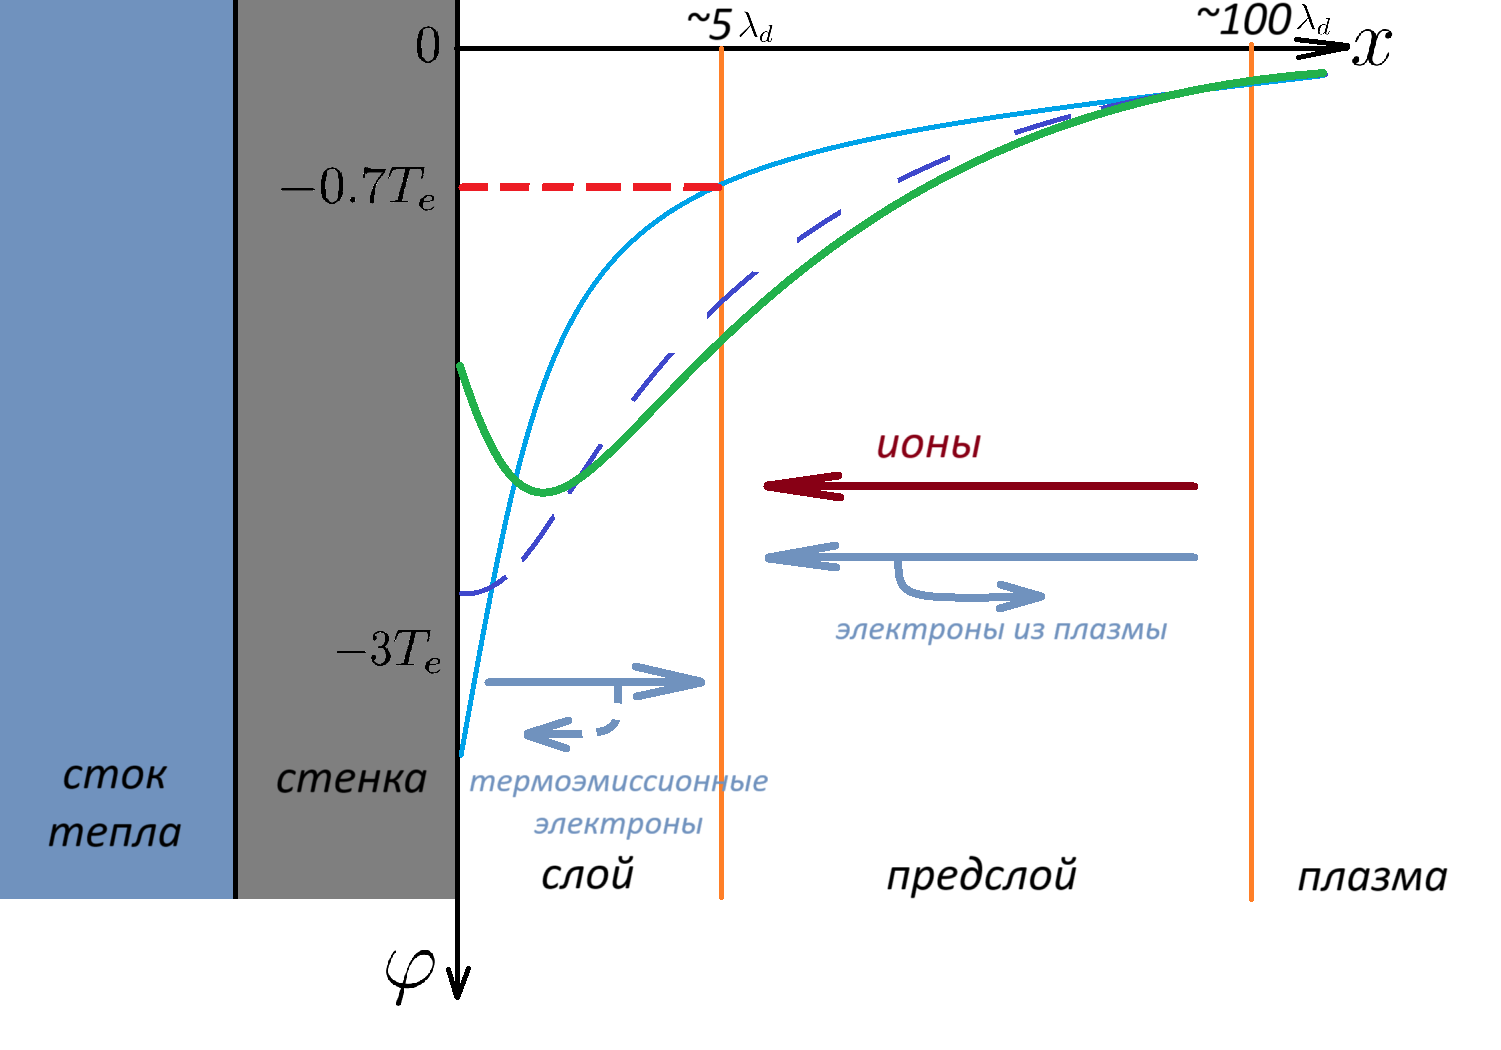
\includegraphics[width=0.7\linewidth]{material/model.png}
	\caption{Модель слоя. Линии соответствуют различным режимам работы: голубая --- классический, фиолетовая прерывистая --- переходный, зеленая --- ограниченный объёмным зарядом. $\lambda_d$ --- радиус Дебая}
	\label{pic::model}
\end{figure}

\qquadТермоэлектронная эмиссия описывается законом Ричардсона---Дешмена. В работе так же рассмотрено влияние эффекта Шоттки~\eqref{eq::Shottky}:
\begin{subequations}
    \begin{align}
        j_{te} &= aT_s^2\exp{\cfrac{-e(\varphi_{out} + \Delta\varphi_{Sh})}{T_s}}
        \\ \Delta\varphi_{Sh} &= -\sgn{E_x}\cdot\sqrt{e\lvert E_x\rvert}
    \end{align}
    \label{eq::Shottky}
\end{subequations}


\qquadОбразовавшаяся структура может быть разделена на \\несколько областей: у стенки находится дебаевский слой, в котором нарушена квазинейтральность плазмы
и присутствует сильное поле. Для образования данной структуры ионы должны иметь достаточно большую скорость, которую они набирают
в предслое --- области между плазмой и слоем. 
Значение потенциала входа в дебаевской слой не равно нулю. Уменьшение потенциала соответствует разгону 
ионов до скорости $\upsilon_0$, требуемой для выполнения критерия Бома~\cite{stangeby2000plasma}
существования неосциллирующего решения уравнения Пуассона в слое:
\begin{equation}
	\varphi_{se} = \cfrac{-m_i\upsilon_0^2}{2e}
	\label{eq::Bohm}
\end{equation}

\qquadРазмеры предслоя гораздо больше размеров слоя(порядка $100$ радиусов Дебая для предслоя, $\sim 5$ --- для слоя)

\qquadВ работе рассмотрены следующие режимы:
\begin{itemize}
    \item Классический --- присутствует поле возле стенки, поле в слое монотонно возрастает
    \item Ограниченный объёмным зарядом --- ввиду активной эмиссии электронов со стенки возникает виртуальный катод в слое, приводящий к экранированию потока термоэмиссионных электронов
\end{itemize}

